\chapter[Experimental approaches]{Experimental approaches to the prosody of Totoli}
\label{sec:Experiments}


\citet[250]{himmelmann2008prosodic}  summarize that sentence-level prosody \is{postlexical prosody} is typically employed in marking sentence modality, \is{modality} phrasing, \is{phrasing} and prominence. \is{prominence} In this chapter, I present experimental evidence that focuses particularly, though not exclusively, on the latter, i.e. the role of prominence \is{prosodic prominence} in the prosody of Totoli. The chapter consists of two sections. In the first section, I present the results of a Rapid Prosody Transcription (RPT) \is{Rapid Prosody Transcription} experiment (\sectref{sec:RPT}). This setup has proven particularly useful for obtaining a first impression of the prosody of a little-known language. The study's results are complemented by two focus marking \is{focus} experiments, which constitute the second section of this chapter (\sectref{sec:Fokus}). This section explores whether prosodic prominence is used to mark the information-structural category focus. \is{information structure} To ensure adherence to the fundamental principle of complete reproducibility,  R scripts and raw data can be readily downloaded from \citet{OSF}. 


\section[Rapid Prosody Transcription experiment]{Investigating the role of prosodic prominence through a Rapid Prosody Transcription experiment}
\label{sec:RPT}

\is{Rapid Prosody Transcription|(}
\is{prosodic prominence|(}

As a first step towards understanding the prosody of Totoli, I conducted a Rapid Prosody Transcription (RPT) experiment to gain preliminary insights into the role of prosodic prominence in the language's intonation. The RPT method is a simple and relatively quick tool that captures listeners' perception of boundaries and prominences \citep{mo2008naive, cole2014listening}.
A description of the method is given by  \citet[11]{Cole2016}.

\begin{quotation}
	[It] draws on linguistic theories of prosody (or intonation) in recognizing prominence and phrasing as two separate dimensions of prosodic form, and as such RPT can be used within any theoretical framework that recognizes prominence and phrasing, as a means of tapping into ordinary listeners’ subjective impression of prominences and boundaries in speech.  
\end{quotation}

In an RPT experiment, speakers are presented with speech samples and a transcription thereof and are asked to identify perceived prominences and boundaries, based on their auditory impression of the recording.  The task does not require any experience in prosodic transcription or linguistic knowledge. The RPT method has been employed in a number of studies on well-researched languages such as \ili{English} \citep{mo2008naive,cole2010signal}, German \citep{riesberg2020}, \ili{Estonian} \citep{Ots_2019}, and \ili{Korean} \citep{you2012determining}. 



Crucial in the choice of RPT as experimental approach towards the prosody of Totoli taken here is \citeauthor{Cole2016}'s  note that it is particularly useful for ``populations not easily accessed from the university communities where most prosody researchers reside [and it] opens the door to obtaining prosody judgments from minority linguistic communities, from elderly people and those in rural communities, and from communities of language learners" (\citeyear[12]{Cole2016}).  \citet{riesberg2018perception, riesberg2020} followed up on this suggestion and successfully employed the RPT method in a study on \ili{Papuan Malay}.


In this light, RPT provides a suitable setup for this investigation here. 









\subsection{Materials}
\label{Materials}

For the experiment, speech samples were taken from recordings of Pear Story \is{Pear Story \citep{chafe1980pear}} \citep{chafe1980pear} retellings from the Totoli language corpus (see  \sectref{IU-Props}). Five different speakers were selected based on the quality of their retelling in terms of smooth speaking flow and naturalness. A total of 71 speech samples were taken from the recordings, each ranging between 1.37 and 6.73 seconds in length and comprising between one and three CIUs.

\tabref{Overview stimuli} gives an overview of the number of CIUs the speech samples contain. 


\begin{table}
	\caption{Number of CIUs contained in the samples used in the RPT experiment}
	\label{Overview stimuli}
	\begin{tabular}{cc}
		\lsptoprule
		Number of  & Number of   \\
		 speech samples &  CIUs in speech sample  \\
		\midrule
		41                       & 1                               \\
		26                       & 2                               \\
		4                        & 3                               \\
		\midrule
		total = 71              	&                                \\
		\lspbottomrule
	\end{tabular}
\end{table}

\tabref{Overvieww stimuli} gives an overview of the number of words and the duration of samples used in the RPT experiment.

\begin{table}
	\caption{Duration (in seconds) and number of words in speech samples}
	\label{Overvieww stimuli}
	\begin{tabular}{l S[table-format=1.2] S[table-format=2.2] S[table-format=1.2] S[table-format=1.2] S[table-format=1.2] S[table-format=3.2]}
		\lsptoprule
		                    & {min}  & {max}  & {mean} & {median} & {sd}   & {total}  \\ \midrule
		number of words     & 4    & 13   & 6.83 & 6      & 2.32 & 484    \\
		duration in seconds & 1.37 & 6.73 & 2.78 & 2.68   & 1.03 & 197.26 \\
		\lspbottomrule
	\end{tabular}
\end{table}

Further information about the speakers of the stimuli is given in  \sectref{sec:rec_spkr-information} of the Appendix.


The speech samples were presented without any punctuation and used the local orthography.  An example is discussed below (see example \REF{ex:isakemo ulang dɛi sapeda} and its realization in \figref{wave form scores example}).





\subsection{Participants}
\label{Participants}



Twenty native Totoli speakers were recruited for the experiment: 12 male and 8 female --- \textit{M\textsubscript{Age}} = 30.05; \textit{Range\textsubscript{Age}} = 18--45.
Participants were required to be fluent in Totoli and possess good computer skills. All participants reported being born and raised in the Tolitoli regency (Kabupaten Tolitoli) and raised with Totoli as their first language. Additionally, they are also fluent speakers of the spoken variety of Indonesian/Malay in the region, and to varying degrees, Standard Indonesian. Further information regarding the participants can be found in  \sectref{sec:participant-information} of the Appendix.


Totoli is an endangered language and, as such, the recruitment of participants is challenging. Consequently, all 20 participants in the experiment were asked to perform both boundary and prominence judgments. To control for potential task order effects, I followed the approach of \citet{mo2008naive} and divided the participants into two groups. The first group rated prominences before boundaries, while the second group completed the tasks in the reverse order.




\subsection{Procedure}
\label{Procedure}


In an RPT experiment, participants are presented with speech samples along with a transcription of the recording and are asked to identify perceived prominences and boundaries based on their auditory impressions. It is noteworthy that the task does not require any experience in prosodic transcription or linguistic knowledge.

The stimuli were presented via the LMEDS \is{LMEDS} web interface \citep[206]{cole2017crowd, mahrt2016lmeds}. Since Indonesian is the national language and the medium of formal education, the instructions were given in Indonesian, as participants would find it highly unnatural to receive instructions in Totoli. To maintain consistency and comparability, the instructions and examples were taken from \citet[409--411]{riesberg2018perception} and reprinted in  \sectref{Instructions boundaries} and \sectref{Instructions prominences} of the Appendix. 



Boundaries were briefly explained to participants as a tool employed by speakers to chunk some words together or separate others (see  \sectref{Instructions boundaries} of the Appendix). An example of grouped numbers in a long telephone number was given: 



\begin{center}
	229 \quad 100 \quad 2999
\end{center}

A second example was given which was equivalent to:\footnote{The Indonesian example given was: \textit{Bapak saya sudah datang.} `My father is already at home.' vs. \textit{Bapak, saya sudah datang.} `Father, I am already home.'; cf. \citet[409--412]{riesberg2018perception}.}


\begin{center}
	\textit{``I eat, Father."} \quad vs. \quad \textit{``I eat father."}
\end{center}

The concept of \textit{prominence}, on the other hand, has no exact equivalent in Indonesian  \citep[compare also ][29]{Cole2016}.  \citet[409]{riesberg2018perception} describe prominences  as a way in which speakers make some words stand  out (Indonesian: \textit{menonjol} `to stand out') and state that this can usually be heard or felt by the listener. The exact wording and a translation to English is reprinted in   \sectref{Instructions prominences} of the Appendix. 


 Two Indonesian examples were presented to the participants; their English translations are reprinted here:

\bigskip

\quad \quad \quad \quad \quad \quad	1) She sees  \BracksEmphasis{{a cow}} 

\medskip


\quad \quad \quad \quad \quad \quad	2) She sees a \BracksEmphasis{{cow}} and a horse  \BracksEmphasis{{eating}} grass

\bigskip






In the LMEDS \is{LMEDS} web interface, speakers click on a word: in the boundary-marking task, a vertical bar  (\textbf{|})  appears after a selected word to indicate a boundary; in the prominence-marking task, the selected word appears in \BracksEmphasis{{bold}}.
Participants listened to the audio exactly twice. Selection of words (i.e. placement of boundaries or prominences) was permitted only after participants had listened to the speech sample at least once. No time constraint was given for marking either the boundaries or prominences for a respective speech sample. Participants were told explicitly that they were free to mark as many or as few boundaries or prominent words as they wanted. They were also told that they could change their minds, selecting and deselecting words freely before continuing to the next speech sample.

The prominence- and boundary-rating tasks are illustrated in example  \REF{ex:isakemo ulang dɛi sapeda}, taken from the speech samples used in the experiment.  The glossing and translation is included here for the reader only and boundary and prominence marking is arbitrarily chosen for the illustration of the task. In the experiments, participants were presented with the transcript --- i.e. the first line --- only.



\ea
\label{ex:isakemo ulang dɛi sapeda}
\textit{isakɛmɔ \BracksEmphasis{{ulaŋ}} dɛi sapɛda maŋana ia  \BracksEmphasis{{nal​lakɔmɔ}}} \\
\textit{isakɛmɔ ulaŋ} \textbf{|} \textit{dɛi sapɛda} \textbf{|} \textit{maŋana ia  nallakɔmɔ} \\ \quad \\
\gll ni-sakɛ-0=mɔ ulaŋ dɛi sapɛda maŋana ia nɔ-\textsc{rdp-}lakɔ=mɔ \\
\textsc{rls}-put.up-\textsc{uv}=\textsc{cpl} again \textsc{loc} bike child \textsc{prx} \textsc{av.rls}-\textsc{rdp}-walk\textsc{=cpl} \\
\glt `(after he) puts it on his bicycle again, the child walks off'
\begin{flushright}(pearstory\_9\_FAH.039-40)
	\osflink{65a54fec1cba3e0c1801854a}{46-isakemo_ulang_dei_sapeda_mangana_ia_nallakomo_pearstory_9_FAH_.wav}\end{flushright}
\z





Before the Totoli data was presented to the participants, they completed a training run with four  Indonesian speech samples taken from Pear Story \is{Pear Story \citep{chafe1980pear}} retellings. Participants had no prior experience in participating in an experiment and the trial runs in a language they are most familiar with as written medium was deemed necessary so that they could get accustomed to the task.  \citet{riesberg2020} showed that participants are very sensitive to language specific cues in the marking of prominences, even in languages they are not familiar with. Based on these results, I do not expect any influence of the trial runs in Indonesian, although a potential influence on the overall result cannot be excluded. 

\subsection{Analysis}
\label{Analysis}

Participants rated 71 speech samples. Boundaries placed after the last word of a given speech sample were discarded, as no judgment was needed there. Following \citet[304]{cole2010signal}, I calculated boundary scores (b-scores) and prominence scores (p-scores) for each word,  representing the proportion of speakers who marked the respective word as prominent or as preceding a boundary. 

In  \figref{scores example}, the results of both tasks are illustrated for the speech sample presented above in example  \REF{ex:isakemo ulang dɛi sapeda}. The speech sample consists of two CIUs.



\begin{figure}
	\includegraphics[width=\textwidth]{figures/example_RPT.png}
	\caption{p-scores and b-scores for example  \REF{ex:isakemo ulang dɛi sapeda}, squared brackets indicate CIU boundaries.}
	\label{scores example}
\end{figure}

Figure \ref{scores example} shows that most speakers perceived a boundary following \textit{sapɛda} ‘bicycle’ (b-score = 90), which coincides with the location of a CIU boundary determined by my analysis (see  \sectref{The units of spoken speech}). Similarly noticeable are the relatively high p-scores for the first word of the first CIU,  \textit{isakɛmɔ} `put up' (p-score = 45), and the last word of the second CIU, \textit{nal​lakɔmɔ} `to go' (p-score = 70). 



\figref{wave form scores example} shows the periogram with pitch track in semitones (st) of example  \REF{ex:isakemo ulang dɛi sapeda}. The pitch contour is given in yellow. The blue line in the background gives information on periodic energy, represented by the width and transparency of the line. The prominence  ratings are indicated in red and the boundary ratings are indicated in black. 

\begin{figure}
	\includegraphics[
	height=0.3\textheight
	%,
	%width=0.99\textwidth
	]{figures/46-isakemo_ulang_dei_sapeda_mangana_ia_nallakomo_pearstory_9_FAH__plot.png}
	\caption{Periogram with pitch track (in st) for example \REF{ex:isakemo ulang dɛi sapeda}: order of tiers from top to bottom is word, p-score, b-score; speaker FAH.}
	\label{wave form scores example}
\end{figure}

%In order to better understand the judgments of boundaries and prominences, I analyzed interrater agreement.

Inspection of the pitch contour given in  \figref{wave form scores example} and its comparison with the respective boundary and prominence ratings in  	\figref{scores example} shows that boundary ratings, prominence ratings and pitch rises appear to largely coincide. 





To analyze the degree of agreement between participants, I calculated Fleiss’ kappa and Cohen’s kappa ($\kappa$) coefficients  \citep{Fleiss_1971, Cohen_1960}.  Cohen's $\kappa$ measures the agreement of judgments between two participants over all rated items, thus providing $(n^2-n)/2$ values for $n$ participants. Fleiss’ $\kappa$ is a measure that provides a single figure indicating the overall agreement among all participants. Kappa values range from 0 to ($-$)1. A value of 0 indicates agreement at chance level and a positive value indicates agreement above chance level \citep[83]{statitstics_dict}. 



First, I discuss the Fleiss’ kappa and Cohen’s kappa for Totoli before relating the results more meaningfully to those reported for other studies.


\subsubsection{Fleiss' kappa coefficients}\label{sec:fleiss-kappa-coefficients-and-z-normalized-scores}

\is{interrater agreement|(}
\is{boundary placement|(}
\is{prominence placement|(}
\is{Fleiss' kappa|(}


 \tabref{Fleiss' kappa scores and z-scores} shows the Fleiss' $\kappa$ coefficients for the boundary-rating task and the prominence-rating task. It provides values for all raters together, as well as separately for the group that rated boundaries first and then prominences and vice versa.



\begin{table}
	\caption{Fleiss' kappa: the difference between rated subjects equals the 71 discarded words in stimulus-final position for boundary ratings.}
	\label{Fleiss' kappa scores and z-scores}
	\begin{tabular}{lll rrr}
		\lsptoprule
		prominences &&            & all   & boundaries first   & prominences first   \\
		\midrule
		& Stimuli &= & 484   & 484   & 484   \\
		& Raters &=   & 20    & 10    & 10    \\
		& \textbf{Kappa}& =    & \textbf{0.143} & 0.138 & 0.165 \\
		%		& z &=        & 43.3  & 20.3  & 24.4  \\
		%		& p-value &=  & 0     & 0     & 0     \\
		\midrule
		boundaries  &&            & all      & boundaries first  & prominences first \\
		\midrule
		& Stimuli  &= & 413     & 413   & 413 \\
		& Raters &=   & 20        & 10  & 10  \\
		& \textbf{Kappa} &=    & \textbf{0.485}  & 0.497& 0.506 \\
		%		& z &=        & 136       & 67.7 & 69 \\
		%		& p-value &=  & 0         & 0  & 0   \\
		\lspbottomrule
	\end{tabular}
\end{table}

Here, I interpret the kappa values only in relation to each other. 
Comparing the values between the two tasks gives information about the extent to which the raters agree on the placement of prominences in comparison to the placement of boundaries. The kappa values in  \tabref{Fleiss' kappa scores and z-scores} are substantially lower for judgments of prominence placement ($\kappa = 0.143$) than for judgments of boundary  placement ($\kappa = 0.485$). 

The comparison of kappa values between the two groups, i.e. those who rated boundaries first and then prominences and vice versa, provides information about the influence of the task order. The comparison shows that, similar to the findings of \citet[736]{mo2008naive}, the influence of order of tasks  does not have a strong effect (prominence placement: $\kappa = 0.138$ and 0.165; boundary placement: 0.497 and 0.506).  


In sum, the participants agreed substantially more on the placement of boundaries than they did on the placement of prominences. The task order, however, had only a marginal effect on the kappa values.

To further  analyze the degree of agreement between individual pairs of speakers,  Cohen's kappa coefficients were calculated.


\is{Fleiss' kappa|)}

\subsubsection{Cohen's kappa coefficients}
\label{sec:cohens-kappa-coefficients-and-z-normalized-scores}

\is{Cohen's kappa|(}



The distribution of Cohen’s kappa coefficients for pairwise interrater agreement between speakers are shown below in the violin plot in   \figref{Distribution of Cohen's kappa coefficients}.





\begin{figure}
	\includegraphics[
	width=0.99\textwidth]{figures/cohens_kappas.png}
	\caption{Distribution of Cohen's kappa coefficients of 190 rater pairs: mean boundaries = 0.49, median boundaries = 0.52; mean prominences = 0.15, median prominences = 0.14}
	\label{Distribution of Cohen's kappa coefficients}
\end{figure}

\figref{Distribution of Cohen's kappa coefficients} shows that the pairwise agreement on boundaries is substantially higher than agreement for prominences. \citet[165]{landis1977measurement} propose agreement bins for the classification of pairwise interrater agreement values.   \figref{Binned agreement TTL} shows the frequency distribution across agreement bins: $<$0.00 = \textit{poor};  0.00--0.20 = \textit{slight}; 0.21--0.40 =  \textit{fair}; 0.41--0.60 = \textit{moderate}; 0.61--0.8 = \textit{substantial}; 0.81--1.00 = \textit{almost perfect}.


\begin{figure}
	\includegraphics[
	%height=0.3\textheight,
	width=\textwidth]{figures/cohens_kappas_bins.png}
	\caption{Frequency distribution of Cohen's kappa coefficients in
		agreement bins according to \citet[165]{landis1977measurement}: total numbers are indicated in brackets.}
	\label{Binned agreement TTL}
\end{figure}

In the case of boundaries,  no pairs are found in the \textit{poor}, 6.84\% in the \textit{slight}  and 16.32\% in the \textit{fair} categories, with the majority being in the category \textit{moderate} (57.37\%). Some are even in the category \textit{substantial} (19.47\%). As for prominences, 79.48\% of all pairs are found in the categories \textit{poor} and \textit{slight}. \textit{Moderate} is only attested for three pairs (1.58\%) and non fall into the category \textit{substantial} or \textit{almost perfect}.

\is{Cohen's kappa|)}

\is{interrater agreement|)}
\is{boundary placement|)}
\is{prominence placement|)}


\subsection{Discussion}
\label{sec:discussion and comparison}

The Fleiss' $\kappa$ and Cohen's $\kappa$ coefficients above show that participants generally agree only very little on the judgment of which word in a given speech sample is prominent. They agree considerably better on the placement of boundaries. This is especially evident when considering the  pairwise interrater agreements of the Cohen's $\kappa$. 


As measurements of interrater agreement, Cohen’s $\kappa$ and Fleiss’ $\kappa$ have been used in a number of RPT studies on different languages, providing a growing body of literature for comparison.   Figures~\ref{Kappa comparison b} and \ref{Kappa comparison p} compare the results obtained for Totoli with those reported by other studies. There are more studies that report on values for agreements on prominence ratings than on boundary ratings. Note, however, that the different studies vary with regard to the speech samples used, which may limit their comparability.

In the studies of American \ili{English} \citep{mo2008naive,cole2010signal}, excerpts from the Buckeye Corpus of spontaneous conversations \citep{Pitt.2007} were used for the  experiment. Similarly, the study of \ili{Papuan Malay}  \citep{riesberg2018perception, riesberg2020} used samples of spontaneous speech, obtained from recordings of the Pear Film \citep{chafe1980pear} and the Tangram Task. The  study on \ili{Estonian} \citep{Ots_2019} used excerpts of the Phonetic Corpus of Estonian Spontaneous Speech.  \citet{you2012determining} used answers obtained from two native speakers replying to a set of questions in \ili{Korean}. Lastly, data on \ili{German} are reported by \citet{Baumann_2018}, who used  sentences  read out loud for the RPT experiment. The study of Totoli is  most comparable to that on \ili{Papuan Malay}  by \citet{riesberg2020} regarding the experimental setup and material used.



\newpage
\figref{Kappa comparison b} shows the Fleiss’ $\kappa$ coefficients of the boundary-rating task reported in the studies mentioned above, comparing these with the results obtained from Totoli. 


\begin{figure}
	\includegraphics[
	%height=0.3\textheight,
	width=0.99\textwidth]{figures/typology_boundaries.png}
	\caption{Fleiss’ $\kappa$ for boundary ratings using the RPT method: dots indicate single reported values, lines indicate reported range.}
	\label{Kappa comparison b}
\end{figure}



 \tabref{Kappa comparison p} shows the Fleiss’ $\kappa$ coefficients reported in  various studies for the prominence-rating task.




\begin{figure}
	\includegraphics[
	%height=0.3\textheight,
	width=0.99\textwidth]{figures/typology_prominences.png}
	\caption{Fleiss’ $\kappa$ for prominence ratings using the RPT method: dots indicate single reported values, lines indicate reported range.}
	\label{Kappa comparison p}
\end{figure}


Across the languages, Fleiss’ $\kappa$ coefficients vary substantially for prominence ratings.  The highest results for agreement were found for \ili{German} with a Fleiss’ $\kappa$ coefficient of 0.53   \citep{Baumann_2018}. The lowest results were reported for \ili{Papuan Malay}  \citep{riesberg2018perception, riesberg2020} with a Fleiss’ $\kappa$ coefficient of only 0.103. The results obtained for Totoli ($\kappa = 0.143$) are similar to that of \ili{Papuan Malay}, although slightly higher.


In sum, the comparison  of prominence and boundary ratings across the various studies on various languages shows a higher degree of agreement for boundary rating than for prominence rating. With regard to boundary rating, the results for Totoli are similar to those reported by other studies (see  \figref{Kappa comparison b}). With regard to prominences, however, Totoli listeners show comparatively low agreement values that are most similar to those reported for \ili{Papuan Malay} (see  \tabref{Kappa comparison p}).  The results point to the fact that prosodic prominence may not be a relevant category in the prosodic system of Totoli. 

This is in fact similar to what \citet{riesberg2018perception} report for \ili{Papuan Malay}, where participants show comparatively low agreement on prominence placement and appear to perceive prominences mainly at boundaries.  \citet[2]{riesberg2020} caution that the results obtained from an RPT study, such as the above, ``cannot establish ‘facts’ of the type ‘language X makes use of pitch accents’ or ‘speakers of language X hear durational differences as marking lexical stress.’" Therefore, I conducted two further experiments, reported in \sectref{sec:Fokus} that  examine the  assumption about a possible lack of prosodic prominence marking in Totoli.

\is{Rapid Prosody Transcription|)}
\is{prosodic prominence|)}

\section[Focus marking experiment]{Investigating the role of prosodic prominence through a focus marking experiment}
\label{sec:Fokus}

\is{focus|(}
\is{focus marking|(}
\is{information structure|(}
\is{prosodic focus marking in Totoli|(}
In order to further investigate the role of prosodic prominence in Totoli, I conducted a production and perception experiment which examines whether focus is acoustically prominent in the marking of information-structural categories, such as focus.





Studies on \ili{West Germanic} languages show a fine-grained distinction between various focus structures, with the most pronounced difference in production between background and \isi{narrow focus} \citep{MUCKE201447, baumann2006prosodic, SWERTS2002629, KALAND2023101200, Lee_2015, 0023830919880217}. Thus, if prosodic prominence were to play a role in the marking of focus in Totoli, I  expect it to be observable in  constructions such as those in  \figref{QA pairs}. 




\begin{figure}
	\caption{Example of question-answer pairs with a syntactically identical answer}
	\label{QA pairs}
	\begin{tikzpicture}[scale=6]
		
		
		\tikzstyle{bla} = [rectangle, rounded corners, minimum width=5cm, minimum height=1.5cm,text centered, draw=black]
		\tikzstyle{bla2} = [rectangle, rounded corners, minimum width=1cm, minimum height=0.7cm,text centered, draw=black]
		\tikzstyle{arrow} = [thick,->,>=stealth]
		
		
		
		
		\node (Q1) [bla]{\begin{tabular}[c]{@{}l@{}}\textbf{\textcolor{blue}{isɛi}} nɔŋinum ɔɡɔ?\\    \textsc{who} \textsc{av.rls}-drink water\\ \\`Who drinks the water?'\end{tabular}};
		\node (Q) [bla2, above of=Q1, yshift = 0.3cm, xshift = -2.5cm] {Question:}; 
		
		\node (A1) [bla,  yshift = -4cm, xshift = 3cm] {\begin{tabular}[c]{@{}l@{}}\textbf{\textcolor{blue}{inaŋ}} nɔŋinum \BracksEmphasis{{ɔɡɔ}}!\\  mother \textsc{av.rls}-drink water\\ \\`The mother drinks water.'\end{tabular}};
		
		\node (A) [bla2, above of=A1, yshift = 0.3cm, xshift = -2.8cm] {Answer:}; 
		
		\node (QQ) [bla2, right of=Q, xshift = 5cm] {Question:}; 
		\node (Q2) [bla, right of=Q1, xshift = 5cm] {\begin{tabular}[c]{@{}l@{}}inaŋ nɔŋinum \BracksEmphasis{{sɔpa}}?\\ mother \textsc{av.rls}-drink \textsc{what}\\ \\`What does the mother drink?'\end{tabular}};
		
		
		\draw [arrow, black]  (Q1.south) --   (A1);
		\draw [arrow, black]  (Q2.south) --   (A1);
		
		
		
	\end{tikzpicture}
	
\end{figure}


Most European languages make use of postlexical pitch accents \is{postlexical pitch accent} as a means to express information-structural categories    \citep[see among others][]{Gussenhoven_1984, Ladd_2008, jun_2014, bolinger1986intonation, Halliday_1967, Grice_English, wagner_2012}. Thus far, little is known about the role of prosodic prominence in the marking of information-structural categories in  \ili{Austronesian} languages. Summarizing what is known so far about \ili{Austronesian} languages of Indonesia, \citet[347]{Himmelmann_Preliminary_2018} comments that ``it seems likely that prosodic prominence does not have a major role to play in marking information-structural categories". 

Inasmuch as is known from typologically diverse languages, phrasing may be an alternative strategy to mark focus: 

\begin{quotation}
	[..] the function of postlexical pitch accent in English  and  other  Germanic  languages  (such  as  marking  focus  or  disambiguating an ambiguous string) is performed by placing words in the same or different prosodic units, i.e. prosodic phrasing in Japanese and Korean. \citep[414]{jun2006_typo} 
\end{quotation} 


As  exemplified in  \figref{QA pairs} above, Totoli allows a syntactically identical clause as an answer to different wh-questions that trigger narrow focus on either the subject or the object. This provides a suitable testing ground for the investigation of focus marking in Totoli and the role of prosodic prominence thereto.


Here, I present an experiment that  examines the role of prosodic prominence in Totoli by searching for prosodic cues in the marking of information-structural categories. \is{information structure} That is, I investigate whether the information structure category of focus \is{focus} is acoustically prominent in identical constructions that were uttered as answers to questions triggering either subject or object focus. 

\subsection{Materials}
\label{sec:materials-focus}

I recorded a set of question-answer (QA) pairs of different focus types (explicated below), taken from  \citet[206--220]{Skopeteas.2006b}. I selected those of narrow focus type for further analysis, including the examples in  \figref{QA pairs}. Different types of narrow focus have been identified; the QA pairs under discussion here correspond to what has been called “information focus”  \citep{krifka2008basic}.  \is{information focus}

I recorded the QA pairs  with 6 different speakers (2 females and 4 males): \textit{M\textsubscript{Age}} = 31.15; \textit{Range\textsubscript{Age}} = 26--61. Further information on the recorded speakers is given in  \sectref{sec:foc_rec-information} of the Appendix. 

The QA pairs were presented to the speakers one by one in a PowerPoint presentation. The recruited speakers had already been recorded beforehand during the Totoli documentation project and, therefore, were  comfortable with the recording setting. All recordings were done in cooperation with Datra Hassan (DT; see Appendix \sectref{sec:foc_rec-information}), native speaker of Totoli and member of the Totoli documentation team. He uttered the questions and the other speakers spoke the answers. The set of QA pairs was recorded twice with each speaker. In the first round, the speakers could familiarize themselves with the task and the different QA pairs. The recordings of this round were not used for the analysis here. Before the second round, the speakers were instructed  to listen attentively to the question to which they were answering. This was done to ensure that, when uttering the answers, speakers were fully aware of the foci triggered by the questions. Speakers were allowed to immediately repeat a QA pair if they judged their production to be unnatural or erroneous.

Both Datra and the speakers were wearing head-mounted AKG C520 condenser microphones, attached to a Zoom Q8 audio/video recorder. Recordings were done at a sampling rate of 44.1 kHz in a 16-bit mono format.




The nine selected QA pairs involved four different answer clauses. Three of the answer clauses were transitive constructions of the structure \textit{subject-verb-object} (SVO) and one of the answer clauses was a ditransitive construction of the structure \textit{subject-verb-object-indirect object} (SVOO\textsubscript{i}). Each of the three transitive clauses occurred twice: once as the answer to a wh-question triggering narrow focus on the subject and once as the answer with narrow focus on the object. The ditransitive clause occurred three times: as the answer to wh-questions triggering narrow focus on the subject, on the object, and on the indirect object.

\begin{table}
	\caption{Type and number of constructions: in-focus constituents are indicated in uppercase letters and colored in blue, constituents that are not in focus are indicated in lowercase letters and colored in yellow.}
	\label{type and number}
	\begin{tabular}{cccc}
		\lsptoprule
		\textsc{type} & \textsc{wh-question}                                                                                           & \textsc{answer type} &\begin{tabular}[c]{@{}c@{}}\textsc{number}\\\textsc{of} \textsc{constructions} \end{tabular}                                                                                                   \\
		\midrule
		transitive    & \begin{tabular}[c]{@{}c@{}} subject focus\\  object focus \end{tabular}                         & \begin{tabular}[c]{@{}c@{}} \textcolor{infocus}{\textbf{S}}\textcolor{verb}{v}\textcolor{outfocus}{o}\\  \textcolor{outfocus}{s}\textcolor{verb}{v}\textcolor{infocus}{O} \end{tabular}                         & 3×\\
		\midrule
		ditransitive  & \begin{tabular}[c]{@{}c@{}} subject focus\\ object focus\\ indirect object focus\end{tabular} & \begin{tabular}[c]{@{}c@{}} \textcolor{infocus}{\textbf{S}}\textcolor{verb}{v}\textcolor{outfocus}{oo\textsubscript{i}}\\ \textcolor{outfocus}{s}\textcolor{verb}{v}\textcolor{infocus}{\textbf{O}}\textcolor{outfocus}{o\textsubscript{i}}\\ \textcolor{outfocus}{s}\textcolor{verb}{v}\textcolor{outfocus}{o}\textcolor{infocus}{\textbf{O\textsubscript{i}}}\end{tabular}&1×  \\
		\lspbottomrule
	\end{tabular}
\end{table}



\begin{figure}
	
	\caption{Example of pairwise analysis of answer pairs: in-focus constituents are indicated in uppercase letters and colored in blue; constituents that are not in focus are indicated in lowercase letters and  colored in yellow.}
	\label{QA pairing1}
	
	\begin{tikzpicture}
		
		
		\tikzstyle{bla} = [rectangle, rounded corners, minimum width=3cm, minimum height=1cm,text centered, draw=black]
		\tikzstyle{arrow} = [thick,->,>=stealth]
		\node (Q1) [bla] {\textcolor{black}{\textbf{What}} is the mother drinking?};
		\node (A1) [bla,  yshift = -2.5cm] {\textcolor{outfocus}{The mother} is drinking \textcolor{infocus}{\textbf{WATER}}!};
		
		
		
		\node (Q2) [bla, right of=Q1, xshift = 5cm] {\textcolor{black}{\textbf{Who}} is drinking the water?};
		\node (A2) [bla, right of=A1, xshift = 5cm] {\textcolor{infocus}{\textbf{THE MOTHER}} is drinking \textcolor{outfocus}{water} !};
		
		\node (speaker1)[bla, above of=A1, minimum height = 0.5cm, minimum width =1cm, xshift=-2cm, yshift=-0.3cm] {Speaker A:};
		\node [bla, right of=speaker1, xshift = 5.1cm, minimum height = 0.5cm, minimum width =1cm] {Speaker A:};

		
		\draw [arrow, black]  (Q1) to (A1);
		\draw [arrow, black]  (Q2)to (A2);
		
	\end{tikzpicture} 
	
	
\end{figure}

For a full account of the set of QA pairs, see \sectref{Prosodyic Prominence Stimuli} of the Appendix.






In the first step (\sectref{sec:Fokus-Acousticanalysis}), I analyzed whether the constituents differ acoustically with regard to focus condition. In the second step (\sectref{sec:Fokus-perception}), I conducted a perception experiment with the goal of investigating whether listeners perceptually distinguish answer pairs such as those in  \figref{QA pairs}. The results of this analysis are explicated below.



\subsection{Acoustic analysis}
\label{sec:Fokus-Acousticanalysis}

Various prosodic cues have been correlated to prosodic prominence \citep[see among others][]{baumann2006prosodic, Maskikit_Essed_2016, Lee_2015, Arnhold2017Model}. For the analysis here, I investigate duration, pitch, and intensity. 


To do so, I first present and discuss data obtained from one randomly selected speaker. Following this, I present and discuss data on the two constituents \textit{ɔɡɔ} ‘water’ and \textit{inaŋ} ‘mother’ as these occur in two different answer clauses --- once in clause-initial subject position and once in clause-final object position --- and in the two different focus conditions.  The two clauses  are given in examples \REF{ex:Inang nonginum ɔɡɔ}  and \REF{ex:ɔɡɔ niinum inang}.


\ea
\label{ex:Inang nonginum ɔɡɔ}
\textit{inaŋ nɔŋinum ɔɡɔ} \\
\gll   inaŋ nɔN-inum ɔɡɔ\\
mother \textsc{av.rls-}drink water\\
\glt `The mother is drinking water.' 
\ex
\label{ex:ɔɡɔ niinum inang}
\textit{ɔɡɔ ni​inum inaŋ} \\
\gll   ɔɡɔ ni-inum inaŋ\\
water \textsc{uv.rls-}drink mother\\
\glt `The mother is drinking water.' \\ \textit{(approx. `The water is being drunk by the mother.')}
\z



The two constructions are a good illustration of the influence of the focus condition on the realization of the constituents in different clause positions, i.e. initial position and final position. The discussion of phonetic parameters is supported by a statistical analysis.

I ran mixed effects models \is{mixed effects model} with the respective parameter as dependent variable and focus as independent variable, using the  \textit{lme4} \is{\textit{lme4}} package \citep{lme4} \is{\textit{lme4}} in \isi{R software} \citep{R_manual}. I included random effects for the speakers, position of the segment and the segments (random intercepts and random slopes). Furthermore, I included the valency of the constructions as a control variable because of the unequal number of observations that I obtained (three recordings for ditransitive constructions and two for transitive constructions).





\subsubsection{Pitch and focus}
\label{sec:pitch-and-focus}



To investigate the effect of focus condition on pitch contour, I measured F0 values   for each constituent of the answer clauses in 30 time steps using Praat software \citep{Praat}. It should be noted that a constituent may consist of a single word, such as \textit{dɛuk} `dog', or multiple words, such as \textit{maŋana dɔlaɡɔ} `the girl'. In a subsequent step, I transformed F0 values to semitones using the \textit{HzToSemitones} command of the Soundgen package \citep{soundgen_R} \is{\textit{Soundgen}} in R software  \is{R software} \citep{R_manual}, with the frequency of the reference value set to 1.


Consider first the pitch contours in  \figref{pitch:pitch inspection}. It displays pitch contours for nine different target constituents produced by a randomly selected speaker (speaker SRN; see  	\tabref{foc_rec_Speaker_RPT}  of the Appendix). Each pitch contour is labeled according to its focus condition (indicated by color) and grammatical role (indicated by a capital letter). For instance, svO denotes a constituent that serves as the object of a transitive clause, while svoO denotes a constituent that serves as the indirect object of a ditransitive clause.


\begin{figure}
	\includegraphics[
	%height=0.4\textheight,
	width=\textwidth]{figures/pitch_inspection.png}
	\caption{Pitch  in st (Ref = 1 Hz) for the target constituents of one randomly selected speaker (SRN): focus condition is indicated by color, for ditransitive constructions, recordings have two elements in the non-focus condition, and one in focus condition, for transitive constructions, each focus condition has one recording; position and clause structure are indicated in brackets, time scale is normalized, phrase position is indicated above the target constituents, position is indicated above the target constituents, position and clause structure is indicated in brackets.}
	\label{pitch:pitch inspection}
\end{figure}



Constituents in clause-initial and clause-medial position show very similar pitch contours in both focus conditions.  For example, the pitch contours of \textit{buuk} (svOo)  `book', \textit{maŋana dɔlaɡɔ} (Svoo)  `girl', \textit{ɔɡɔ} (Svo)  `water', and \textit{dɛuk} (Svo)  `dog' demonstrate no distinguishable influence of the focus condition on their tonal realization, including both the shape of the pitch contours and the pitch range. Noticeably greater variation is attested for elements in final position, such as \textit{dɛi inaŋna} (svoO) `to the mother', \textit{sɛsɛŋ} (svO) `cat', \textit{ɔɡɔ} (svO) `water', and \textit{inaŋ} (svO) `mother'. These elements exhibit more diverse pitch contours, indicating that their tonal realization is more sensitive to the focus condition.



The latter two  occur in both   clause-final position (svO) and  clause-initial position (Svo), cf. example \REF{ex:Inang nonginum ɔɡɔ} and \REF{ex:ɔɡɔ niinum inang} and in both focus conditions (cf.  \figref{QA pairs}). 


\figref{pitch:pitch inspection_position}  shows these two constituents as produced by all speakers. The left-hand column shows their realizations  in clause-initial position and the right-hand column shows their realizations in clause-final position. The focus condition is indicated by color.

\begin{figure}
	\includegraphics[
	%height=0.3\textheight,
	width=0.75\textwidth]{figures/pitch_inspection_position.png}
	\caption{Pitch  in st (Ref = 1 Hz) of the two constituents \textit{inaŋ} `mother' and \textit{ɔɡɔ} `water' in the two focus conditions for all speakers: focus condition is indicated by color, position and clause structure is indicated in brackets, time scale is normalized.}
	\label{pitch:pitch inspection_position}
\end{figure}



Once again, the pitch contours of the two constituents in clause-initial position exhibit very similar shapes across the two focus conditions. However, the constituents \textit{ɔɡɔ} ‘water’ and \textit{inaŋ} `mother' in initial position display variations in the timing of the pitch rise. Specifically, the constituent \textit{ɔɡɔ} ‘water’ exhibits an initial fall or level tone, a steep rise, and a final pitch plateau, while the constituent \textit{inaŋ} `mother' shows a relatively continuous rise. Further investigation is required to determine how the segmental material of the two constituents influences the different pitch contours in initial position. Furthermore, constituents in final position, in the right-hand column, exhibit much greater variability. Notably, a final rising boundary tone and a final rise-fall boundary tone are clearly visible (see  \sectref{sec:tonal-events-at-the-boundaries-of-ius}). The different boundary tones may potentially be correlated with focus marking and could serve as a cue to indicate the focus condition of clause-final constituents.  \tabref{interaction} correlates the IU-final boundary tones used with each focus condition.

\begin{table}
	\caption{IU-final boundary tones per focus condition (n=54 constituents in final position)}
	\label{interaction}
	\begin{tabular}{lccl}
		\lsptoprule
		& final rise-fall  & final rise & total \\
		\midrule
		not in focus  & 12    & 18   &30 \\
		in focus & 10     & 14  & 24\\
		\midrule
		& 22    &  32&=54\\
		\lspbottomrule
	\end{tabular}
\end{table}



An inspection of the boundary tone of the 54 CIUs revealed that out of 30 instances of a constituent in clause-final position not in focus, 12 were produced with a final rise-fall contour, while 18 had a final rise contour. For constituents in final position and in focus, out of 24 instances, 10 had a final rise-fall contour, and 14 had a final rise contour. Due to the small sample size, a correlation between final pitch movement and focus condition cannot be conclusively established. However, while it cannot be completely ruled out, if focus were indeed expressed by the CIU-final boundary complex, a stronger correlation would be expected. Hence, the findings suggest that the choice of final boundary tone does not  indicate the presence or absence of focus.

%A note on phrasing is in order. 
Inasmuch as focus can be expressed by prosodic phrasing in the constructions used here, it involves variation in the chunking of Compound IUs into embedded IUs (cf.  \sectref{IU-model}). In general, a subject in preverbal position is chunked into its own IU, and variation pertains mainly to chunking the verb and a following object NP into either one IU or two separate IUs,  i.e. [ɔɡɔ]\textsubscript{IU} [ni​inum inaŋ]\textsubscript{IU} vs. [ɔɡɔ]\textsubscript{IU} [ni​inum]\textsubscript{IU} [inaŋ]\textsubscript{IU}. 
These two possible realizations are shown in  \figref{ɔɡɔ_niinum_inang1} and  \figref{ɔɡɔ_niinum_inang2}, respectively.



In both realizations the subject \textit{ɔɡɔ} ‘water’ is chunked into its own IU, clearly visible by the pitch rise on the last syllable \textit{.ɡɔ}. In  \figref{ɔɡɔ_niinum_inang1}, the verb \textit{ni​inum} ‘is being drunk’ and the object NP \textit{inaŋ} ‘mother’ are chunked into one IU. In  \figref{ɔɡɔ_niinum_inang2}, however, the verb occurs in a separate IU, indicated by the pitch rise on the final syllable \textit{.num}.


\begin{figure}
	\includegraphics[
	height=0.3\textheight
	%,
	%width=1\textwidth
	]{figures/ogo_niinum_-inang-_QUIS-focus-QAPairs_DT-IFS_2_extIFS_plot.png}
	\caption{Periogram with pitch track (in st) for example \REF{ex:ɔɡɔ niinum inang} with narrow focus on the final constituent \textit{inaŋ} `mother': speaker IFS \osflink{65a55045c585fd0c409ce98e}{ogo_niinum_-INANG-_QUIS-focus-QAPairs_DT-IFS_2_extIFS.wav} }
	\label{ɔɡɔ_niinum_inang1}
\end{figure}


\begin{figure}
	\includegraphics[
	height=0.3\textheight
	%,
	%width=1\textwidth
	]{figures/-ogo-_niinum_inang_QUIS-focus-QAPairs_DT-IFS_2_extIFS_plot.png}
	\caption{Periogram with pitch track (in st) for example \REF{ex:ɔɡɔ niinum inang} with narrow focus on the initial constituent \textit{ɔɡɔ} `water': speaker IFS \osflink{65a55046f2240f0b5032e6ed}{-OGO-_niinum_inang_QUIS-focus-QAPairs_DT-IFS_2_extIFS.wav}}
	\label{ɔɡɔ_niinum_inang2}
\end{figure}










Example \REF{ex:ɔɡɔ niinum inang} and its two realizations in  \figref{ɔɡɔ_niinum_inang1}
and  \figref{ɔɡɔ_niinum_inang2}
 indicate that speakers have a certain freedom with regard to  chunking.  Of 54 clauses, however, the realization in  \figref{ɔɡɔ_niinum_inang2} is the only instance in which a speaker chunks the verb into a separate IU. All other instances lump the verb in an IU together with the following object NP, as in  	\figref{ɔɡɔ_niinum_inang1}. Hence, in the recorded target clauses, focus is not expressed through phrasing or chunking of constituents into IUs. 





To statistically test the influence of the focus condition on pitch, I calculated the  pitch minimum,  pitch maximum, and pitch range as the difference between the maximum and minimum pitch values for each target constituent (subject, direct object, indirect object) in all the target clauses. Mean F0 values were measured for each labeled vowel in the respective constituents to avoid octave jumps. F0 values were then converted to semitones to control for speaker-dependent vocal range.



The outcome of the \isi{mixed effects model }(see \sectref{sec:Fokus-Acousticanalysis}) is given in  \tabref{lmer_pitch}.



\begin{table}
\caption{Results of the mixed effects model with focus as independent variable and pitch range, pitch minimum and pitch maximum as dependent variables}\label{lmer_pitch}
\begin{tabular}{l S[table-format=-1.3] S[table-format=1.3] S[table-format=-1.3] S[table-format=1.3] }
	\lsptoprule
	      & {Estimate} & {SE} & {$t$} & {$\text{Pr}(>|t|)$}\\\midrule
	range & 0.313 & 0.39    & -0.793 & 0.442\\ 
	max  & 0.028  & 0.830   & 0.034  & 0.976\\
	min  & 0.657  & 0.942   & 0.697  & 0.555\\
	\lspbottomrule             
\end{tabular}
\end{table}

The results of the model in  \tabref{lmer_pitch} show that there is no statistically significant effect of focus condition on pitch range, pitch maximum, nor on pitch minimum. Furthermore, the results indicate that the target constituents are produced with a reduced pitch range ($-0.313$ st), and higher pitch maximum (+0.028 st) and minimum (+0.657 st) when in focus.  The effects  are negligible, considering that the \textit{just noticeable difference} (\textit{j.n.d.})  is estimated to be around 1.5--2 st \citep[29]{_t_Hart_1981,Hart_1990}. 

I conclude that the focus condition has no discernible impact on the pitch contour, the pitch minimum and maximum, and pitch range.


\subsubsection{Duration and focus}
\label{sec:duration-and-focus}

To discover any potential effect of focus on duration, I measured the duration from the onset until the end of each labeled constituent.

Similar to the above, I plotted the duration of the nine different constituents in both focus conditions  produced by one randomly selected speaker (speaker ZHRM; cf.  \tabref{foc_rec_Speaker_RPT} of the Appendix). These are given in  \figref{dur inspection_1_speaker}. No apparent effect of focus condition on duration is discernible.



\begin{figure}
	\includegraphics[
	%height=0.3\textheight,
	width=\textwidth]{figures/dur_inspection_1.png}
	\caption{Duration (in seconds) and focus condition of the target words for one randomly selected speaker (speaker ZHRM): for ditransitive constructions, two elements in the non-focus condition, and one in focus condition were recorded; for transitive constructions, each focus condition has one recording; position and clause structure are indicated in brackets.}
	\label{dur inspection_1_speaker}
\end{figure}

The constituents \textit{bu​uk} (svOo) ‘book’, \textit{maŋana dɔlaɡɔ} (Svoo)‘the girl’ and \textit{inaŋ} (Svo) ‘mother’ show very similar values for both focus conditions. With regard to the constituent \textit{ɔɡɔ} (Svo/svO) ‘water’, duration is longer when in focus, especially when in object position (svO). On the other hand, \textit{sɛsɛŋ} (svO) ‘cat’ shows shorter duration when in focus.

To get a better picture of any systematicity across speakers, I plotted durational values for the two words \textit{inaŋ} `mother' and \textit{ɔɡɔ} `water'  produced by all speakers in  \figref{dur inspection_all}.  



\begin{figure}
	\includegraphics[
	%height=0.3\textheight,
	width=0.9\textwidth]{figures/dur_inspection.png}
	\caption{Duration (in seconds) and focus condition of the two constituents \textit{inaŋ} `mother' and \textit{ɔɡɔ} `water' in the two focus conditions  for all speakers; position and clause structure are indicated in brackets.}
	\label{dur inspection_all}
\end{figure}

\figref{dur inspection_all} yields results similar to those obtained from the inspection of pitch contours in   \figref{pitch:pitch inspection_position}.
There appears to be a substantial effect of clause position. Elements in clause-final position are longer than elements in clause-initial position. This is indeed expected  \citep[cf. utterance-final lengthening\slash preboundary lengthening;][]{turk2020speech, byrd2006far, berkovits1993utterance}. However, the focus condition does not yield any apparent effect. The results of the mixed effects model (see \sectref{sec:Fokus-Acousticanalysis}) are given in  	\tabref{lmer_dur}.

\begin{table}
	\caption{Estimate of the group difference of the mixed effects model with focus as independent variable and duration as dependent variable}
	\label{lmer_dur}
	\begin{tabular}{cccc}
		\lsptoprule
		{Estimate}   & {SE} & {$t$}  & $\text{Pr}(>|t|)$ \\
		\midrule
		0.009 & 0.014 & 0.646 & 0.523      \\
		%	\midrule
		%	excl. valency	&0.009 & 0.014 & 0.657 & 0.516      \\
		\lspbottomrule     
	\end{tabular}
\end{table}

The results of the \isi{mixed effects model }show that the effect of focus condition on duration is not significant ($p=0.523$). 

%(The exclusion of valency as control variable has no noticeable impact on the effect of the focus condition on duration; estimate = 0.009; $p$=0.516). 





\subsubsection{Intensity and focus}
\label{sec:intensity-and-focus}

Lastly, I investigated whether there is any potential effect of the focus condition on intensity. I measured the mean intensity in decibels (dB) of each labeled constituent from the onset until the end of the constituent.   As explained above, all recordings were done with head-mounted microphones in order to keep the distance from the microphone to the mouth constant (see  \sectref{sec:materials-focus}). This is a necessary prerequisite for taking into account intensity. No normalization of data is needed as I am visually comparing individual speaker variation and the statistical model includes random effects for speakers.

\figref{intensity_inspect_1} shows the intensity values of the nine different constituents in both focus conditions as produced by one randomly selected speaker (speaker SP; cf.  	\tabref{foc_rec_Speaker_RPT} of the Appendix).


\begin{figure}
	\includegraphics[
	%height=0.3\textheight,
	width=0.9\textwidth]{figures/intensity_inspection_1.png}
	\caption{Intensity (in dB) and focus condition of the target words by one randomly selected speaker (SP): for ditransitive constructions, two elements of the non-focus condition, and one in-focus condition were recorded; for transitive constructions, each focus condition has one recording; position and clause structure are indicated in brackets.}
	\label{intensity_inspect_1}
\end{figure}

\figref{intensity_inspect_1} shows that this speaker tends to produce the constituents in focus with a slightly lower mean intensity, with the exception of  \textit{dɛuk} (Svo) `dog' and \textit{ɔɡɔ} (svO) `water'. 

To see whether this trend can be observed for other speakers as well, I plotted mean intensity values for the two constituents  \textit{inaŋ} `mother' and \textit{ɔɡɔ} `water' of all speakers in  \figref{intensity_inspection_all}.


\begin{figure}
	\includegraphics[
	%height=0.3\textheight,
	width=0.7\textwidth]{figures/intensity_inspection_.png}
	\caption{Intensity (in dB) for the two constituents \textit{inaŋ} ‘mother’ and \textit{ɔɡɔ} ‘water’ in the two focus conditions; position and clause structure are indicated in brackets.}
	\label{intensity_inspection_all}
\end{figure}

\figref{intensity_inspection_all} shows that  the constituent \textit{ɔɡɔ} (svO) `water'  appears to generally be uttered with a slightly higher mean intensity when in focus. In initial position,  mean intensity tends to be lower when in focus (with one exception). No such trend is found for the constituent \textit{inaŋ} ‘mother’.

Again, also with regard to mean intensity, no clear effect of the focus condition is discernible. The results of the mixed effects model (see \sectref{sec:Fokus-Acousticanalysis}) are given in  	\tabref{lmer_intens}.

\begin{table}
	\caption{Results of the mixed effects model with focus as independent variable and intensity as dependent variable}
	\label{lmer_intens}
	\begin{tabular}{cccc}
		\lsptoprule
		Estimate   & SE & $t$  & $\text{Pr}(>|t|)$ \\
		\midrule
		0.601 & 0.909 & 0.661& 0.518    \\
		\lspbottomrule     
	\end{tabular}
\end{table}



The results of the \isi{mixed effects model} show that there is no statistically significant effect of focus on intensity. 



\subsubsection{Summary}

The results of the acoustic analysis suggest that, in the set of clauses analyzed, focus is not prosodically encoded by the parameters tested, i.e. by pitch range, minimum and maximum, CIU-final boundary-tone complexes, phrasing, duration or mean intensity. 

However, the focus condition may be expressed by other means not tested here, for example spectral tilt, variations in the tonal realization of constituents, vowel quality etc. To exclude this possibility, I conducted a perception experiment to see whether native speakers distinguish between different focus conditions.

\subsection{Perception experiment}
\label{sec:Fokus-perception}


In the perception experiment, participants listened to two QA pairs. For the question, the same recording was used in both. The answers, however, although syntactically identical, were previously recorded as answers to different wh-questions that trigger different foci. Hence, in one of the two QA pairs, the answer was the one originally uttered in response to that particular question. In the other QA pair, there was a mismatch (\figref{QA pairing}). In a two-alternative forced-choice experiment, participants were asked to identify the correctly matched QA pair. I expected this to be a particularly easy task if focus is encoded in the answer clauses.





\subsubsection{Participants}



Twenty participants were recruited from the Totoli community, with the prerequisite that they were fluent speakers of the language and sufficiently knowledgeable with computers: \textit{M\textsubscript{Age}} = 32.25; \textit{Range\textsubscript{Age}} = 20--46. All speakers stated that they were born and raised in the  Tolitoli regency (Kabupaten Tolitoli) and were raised with Totoli. As is the default in the area, they are also fluent speakers of the local variety of \ili{Indonesian}/\ili{Malay}  and, to varying degrees, of Standard \ili{Indonesian}. Further information about the participants is given in  \sectref{sec:foc_participant-information} of the Appendix. 




\subsubsection{Procedure}


Participants  listened to one correctly paired QA pair and one incorrectly paired QA pair.  

The experiment was run on a laptop, using the OpenSesame platform \citep{mathot2012opensesame}.  Participants were told that they would hear two QA pairs, of which one was correct and one was incorrect. Their task was to choose the QA pair they perceived as correct. They listened to the two QA pairs twice before making their choice. The task was repeated 72 times per participant (20 participants × 72 choices = 1440). Stimuli were presented in random order and the visual order of the two choices was randomized as well. 
\figref{Illustration of Experiment} illustrates the experimental setup.


\begin{figure}
	\caption{Illustration of experiment procedure}
	\label{Illustration of Experiment}
	
	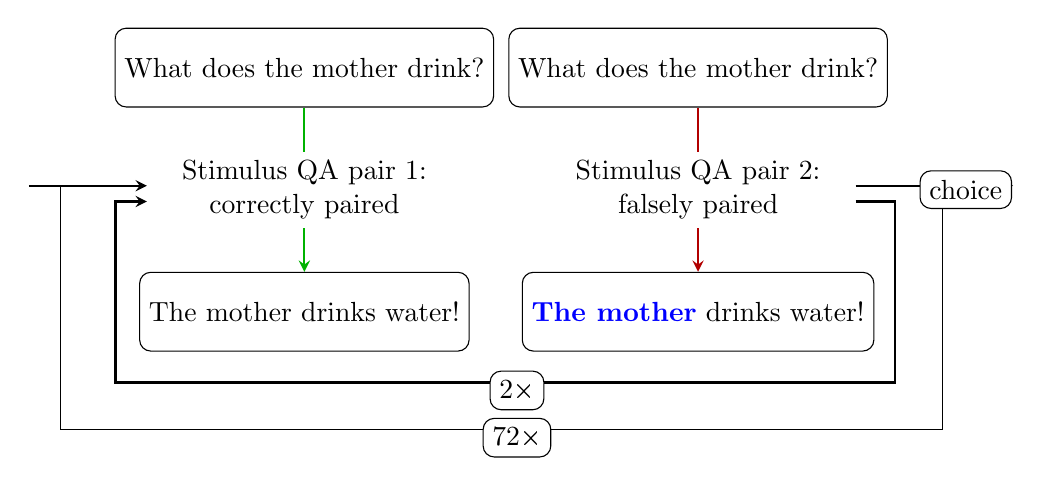
\begin{tikzpicture}
		
		\tikzstyle{bla} = [rectangle, rounded corners, minimum width=4cm, minimum height=1cm,text centered, draw=black]
		\tikzstyle{arrow} = [thick,->,>=stealth]
		
		\node (Q1) [bla] {\BracksEmphasis{{What}} does the mother drink?};
		\node (A1) [bla,  yshift = -3.1cm] {The mother drinks \BracksEmphasis{{water}}!};
		
		
		
		\node (Q2) [bla, right of=Q1, xshift = 4cm] {\BracksEmphasis{{What}} does the mother drink?};
		\node (A2) [bla, right of=A1, xshift = 4 cm] {\textbf{\textcolor{blue}{The mother}} drinks water!};
		
		
		
		\draw [arrow, black!30!green] (Q1) --  node (blub) [black, fill=white, align=center]{Stimulus QA pair 1:\\correctly paired} (A1);
		\draw [arrow, black!30!red]  (Q2) --   node (bla) [black, fill=white, align=center]{Stimulus QA pair 2:\\falsely paired}(A2);
		
		\draw  [arrow] (7,-1.7) -- (7.5,-1.7) -- (7.5,-4) -- (-2.4,-4) -- (-2.4,-1.7) -- (-2,-1.7);
		
		\draw    (8.1,-1.5) -- (8.1,-4.6) -- (-3.1,-4.6) -- (-3.1,-1.5) ;
		
		\draw  [arrow]  (7,-1.5) -- (9,-1.5);
		\draw  [arrow]  (-3.5,-1.5) -- (-2,-1.5);	
		\node[rectangle,fill=white, rounded corners,text centered, draw=black, right of =A2, xshift=-3.3cm, yshift=-1cm]   {2×};
		\node[rectangle,fill=white, rounded corners,text centered, draw=black, right of =A2, xshift=-3.3cm, yshift=-1.6cm]   {72×};
		\node[rectangle,fill=white, rounded corners,text centered, draw=black, right of =A2, xshift=2.4cm, yshift=1.55cm] {choice}  ;
		
	\end{tikzpicture}
	
	
	
	
\end{figure}




\subsubsection{Stimulus preparation}\label{sec:stimulus-preparation}

I used two recordings of each transitive clause: one was previously uttered as the answer to the wh-question triggering focus on the subject, the other was uttered as the answer to the wh-question triggering focus on the object. For the ditransitive clauses, I had three recordings per speaker, each uttered in response to a different question that triggered focus on each of the three constituents. The constructions were summarized in  	\tabref{type and number} in  \sectref{sec:materials-focus}. These constructions were recorded with 6 different speakers, yielding 56 recorded QA pairs of which the answers were cut out.


For the experiment, I combined the same question with two different answers, yielding two QA pairs.


\begin{enumerate}
	\item 	One QA pair consisted of a question paired with an answer that had been previously recorded as the answer to the same question. For instance, a wh-question that triggered focus on the subject was paired with an answer that had been previously recorded in response to a wh-question that also triggered focus on the subject. This resulted in a correctly paired QA pair.
	\item 	The other QA pair was composed of the same question paired with an answer that had been previously recorded as the answer to a question triggering a different focus. For example, a wh-question that triggers focus on the subject was paired with an answer that had been previously recorded as the answer to a wh-question triggering focus on the object. This means that it was an incorrectly paired QA pair.
\end{enumerate}




The pairing of the question with the two answers is exemplified in  \figref{QA pairing}

\begin{figure}
	\caption{Example of pairing of questions and answers}
	\label{QA pairing}
	
	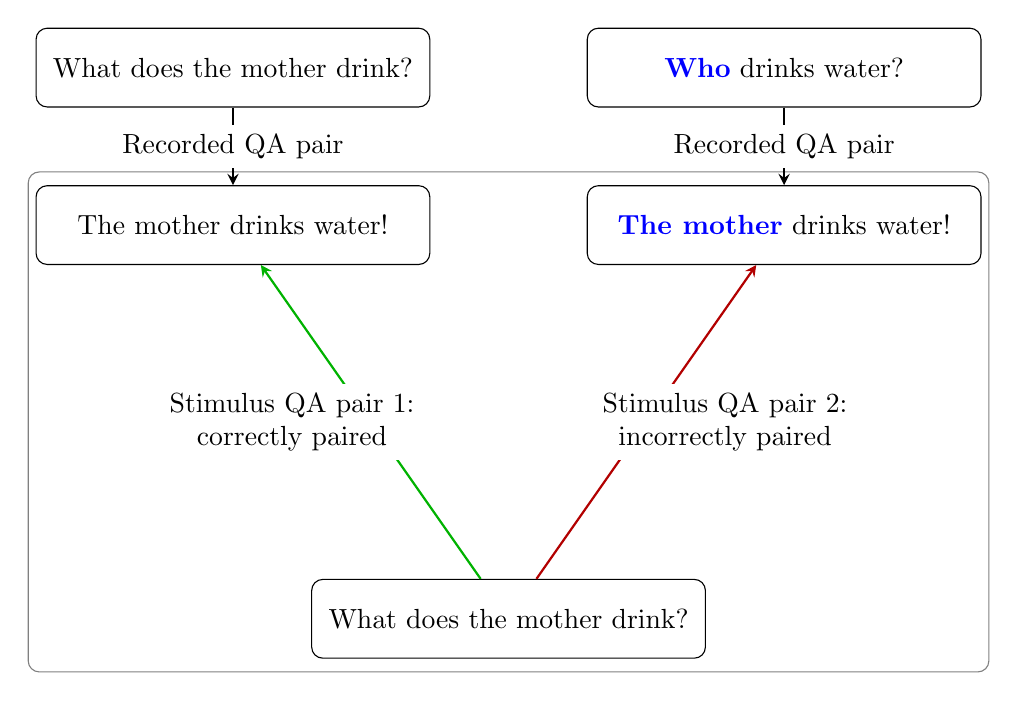
\begin{tikzpicture}
		
		\tikzstyle{bla} = [rectangle, rounded corners, minimum width=5cm, minimum height=1cm,text centered, draw=black]
		\tikzstyle{arrow} = [thick,->,>=stealth]
		
		\node (Q1) [bla] {\BracksEmphasis{{What}} does the mother drink?};
		\node (A1) [bla,  yshift = -2cm] {The mother drinks \BracksEmphasis{{water}}!};
		
		
		
		\node (Q2) [bla, right of=Q1, xshift = 6cm] {\textbf{\textcolor{blue}{Who}} drinks water?};
		\node (A2) [bla, right of=A1, xshift = 6cm] {\textbf{\textcolor{blue}{The mother}} drinks water!};
		\node (QA_blue) [bla, minimum width = 12.2cm, minimum height = 6.35cm, right of =A1, xshift=2.5cm, yshift=-2.5cm, draw=gray]{};
		
		
		
		\node (FQ1) [bla, above of=Q1, yshift = -8cm, xshift = 3.5cm] {\BracksEmphasis{{What}} does the mother drink?};
		
		\draw [arrow, black!30!green] (FQ1) --  node [black, fill=white, align=center, xshift = -1cm]{Stimulus QA pair 1:\\correctly paired} (A1);
		\draw [arrow, black!30!red]  (FQ1) --   node [black, fill=white, align=center, xshift = 1cm]{Stimulus QA pair 2:\\incorrectly paired}(A2);
		\draw [arrow, black]  (Q1) --   node [black, fill=white, align=center]{Recorded QA pair}(A1);
		\draw [arrow, black]  (Q2) --   node [black, fill=white, align=center]{Recorded QA pair}(A2);
		
	\end{tikzpicture}
	
\end{figure}




For the pairing of questions and answers in the perception experiment, all recorded answers from the QA pairs of \sectref{sec:materials-focus}  were used. The pairing was automatically generated and the order was randomized using the OpenSesame \is{OpenSesame} platform \citep{mathot2012opensesame}. To control for speaker variation as a potential factor influencing the choice of the correct QA pair, both choices of answers were taken from recordings of the same person. However, the recorded speaker of the question was always different from the one who recorded the answer to create a natural situation where the questioner and answerer are different individuals.






\subsubsection{Results}
\label{sec:results}



The question at hand is whether participants exhibit a significant preference for the correctly paired QA pair over the incorrectly paired items (chance level = 50\%). If so, it can be assumed that the answer clauses carry prosodic cues that encode information about focus. In other words, if the prosody of Totoli encodes focus, then participants should show a preference for the correctly paired QA pairs. The distribution of question-answer assignments is depicted in \figref{results_experiment_focus}, which reveals that 52\% of participants selected the correctly paired QA pair while 48\% selected the incorrectly paired QA pair.


\begin{figure}
	\includegraphics[
	%height=0.3\textheight,
	width=0.4\textwidth]{figures/results_experiment_focus.png}
	\caption{Distribution of question-answer assignments: horizontal line indicates chance level 50\%, $n = 1440$.}
	\label{results_experiment_focus}
\end{figure}




In order to determine the significance of the participants' tendency to choose the correct answer, I conducted a logistic mixed effects model \is{logistic mixed effects model}  with the choice of QA pair as the dependent variable. The model did not include any predictors. In this case, the intercept is the only parameter of interest, as it measures the probability of choosing the correct answer, with an intercept of 0 on the logit scale representing 50\%. As random intercepts, I included the rater and recorded speaker, as well as the focus type (see \tabref{type and number})). I used  \textit{glmer}() \is{\textit{glmer}} with \textit{family = binomial} of the \textit{lme4} \is{\textit{lme4}} package \citep{lme4} in R \is{R software} \citep{R_manual}.

glmer(), with family = binomial,

The estimate of the intercept was very close to 0 (0.077), indicating only a slight preference for the correctly paired QA pair. This result was not significantly different from 0 ($p = 0.183$; $\text{SE} = 0.058$; $z = 1.332$). Based on these findings, I concluded that the tendency to select the correctly paired QA pair was likely due to chance.




To further investigate participant performance, I analyzed whether there were any observable effects. Specifically, I wanted to determine whether some participants performed differently than others, whether participant performance depended on the recorded speaker, and whether performance varied depending on the position and grammatical role of the constituent in focus.


\subsubsubsection{Effect of rater}


First, I analyzed  the distribution of the question-answer assignment across participants. The results are shown in  \figref{results_experiment_focus_by_rater}.


\begin{figure}
	\includegraphics[
	%height=0.27\textheight, 			
	width=1\textwidth]{figures/results_experiment_focus_by_rater.pdf}
	\caption{Distribution of question-answer assignments by rater: horizontal line indicates chance level 50\%.}
	\label{results_experiment_focus_by_rater}	
\end{figure}

\figref{results_experiment_focus_by_rater} shows that the performance  is comparable across participants. 



One participant (rater 1) showed a particularly high frequency of selecting the correctly paired QA pair (in 69\% of all instances), while another participant (rater 20) showed a higher preference for the incorrectly paired QA pair (in 39\% of all instances).


\subsubsubsection{Effect of recorded speakers}




Second, I analyzed the distribution of the question-answer assignment according to the recorded speaker of the answers of the QA pairs. The results are plotted in  \figref{results_experiment_focus_by_speaker}. Note that the QA pairs were paired such that the answer in both was uttered by the same speaker (cf.  \sectref{sec:stimulus-preparation}).


\begin{figure}
	\includegraphics[
	%height=0.3\textheight, 			
	width=0.6\textwidth]{figures/results_experiment_focus_by_recorded.png}
	\caption{Distribution of question-answer assignments by recorded speaker: vertical horizontal line indicates chance level 50\%.}
	\label{results_experiment_focus_by_speaker}	
\end{figure}

\figref{results_experiment_focus_by_speaker} shows that there is  only slight variation in task performance depending on the recorded speaker. The differences appear to be  negligible. 





\subsubsubsection{Effect of position}





Thirdly, I investigated the distribution of the question-answer assignment according to the position in the clause of the constituent that is focused by the question. The results are plotted in  	\figref{Correct answers by grammatical role of focused constituent}.	

\begin{figure}
	\includegraphics[
	%height=0.3\textheight, 
	width=0.6\textwidth]{figures/results_experiment_focus_by_target_of_q.png}
	\caption{Distribution of question-answer assignments by position of the in-focus constituent in the clause: medial position means the direct object of ditransitive constructions (svOo), final position means the indirect object of ditransitive constructions and the object of the transitive constructions (svO/svoO); horizontal line indicates chance level 50\%.}
	\label{Correct answers by grammatical role of focused constituent}	
\end{figure}

\figref{Correct answers by grammatical role of focused constituent} shows that the position in the clause of the constituent that is focused by the question does not affect performance in choosing the correctly paired QA pair.


\subsubsubsection{Summary}




The data exploration examined three factors that may have influenced the question-answer assignment performance: rater, recorded speaker, and position in the clause of the constituent on which the question triggers focus. Despite some variability, particularly with individual raters, the analysis revealed that none of these factors had a significant impact on participants' performance.


\subsection{Discussion}
\label{sec:conclusion}
In this section, I presented an experimental analysis of the interaction of prosody and focus in Totoli. To this end, I presented an experiment that  examines the role of prosodic prominence in Totoli by searching for prosodic cues in the marking of information-structural categories. 

The topic was first approached  by an investigation that analyzed whether the information-structural category of focus is acoustically prominent in identical constructions that were uttered as answers to questions triggering either subject or object focus (\sectref{sec:Fokus-Acousticanalysis}). The following section described a perception experiment to investigate whether native speakers distinguish between different focus conditions (\sectref{sec:Fokus-perception}).

In order to investigate the effect of focus condition on the production of syntactically identical constructions, I analyzed the phonetic parameters related to pitch, duration, and intensity (\sectref{sec:pitch-and-focus}--\sectref{sec:intensity-and-focus}). However, no significant effect of the focus condition was observed in any of these parameters.  To exclude the possibility of focus condition  being expressed by other means not tested here, I conducted a perception experiment to see whether native speakers distinguish between different focus conditions (\sectref{sec:Fokus-perception}). However, the results of the perception experiment revealed no significant difference in the perception of syntactically identical clauses recorded as answers to questions with different foci. Based on these findings, I conclude that focus is not prosodically encoded in the set of clauses analyzed.

\is{syntactic focus marking in Totoli|(}


As the present investigation focuses on a controlled experimental analysis of focus marking in Totoli, it is important to note that in less controlled situations, speakers of Totoli use syntactic means and concomitant prosodic phrasing to express focus. While an in-depth investigation of this focus marking strategy is beyond the scope of this study, two examples are provided for illustration purposes. These instances are taken from a recording of an adapted version of the Anima elicitation game described in \citet[99--107]{Skopeteas.2006b}, which was originally designed to elicit different focus types. In this game, participants are shown pictures and then asked questions about them. Examples \REF{ex:Oto ana focus} and \REF{ex:Moane anu focus}  illustrate focus marking in Totoli in this less controlled setting.



In example \REF{ex:Oto ana focus}, the speaker answers to a question asking about the patient of the situation (``\textit{In front of the well}: \underline{What} is the man pushing?";  adapted from \citealt[103]{Skopeteas.2006b}). 
The speaker replies with a cleft construction in order to mark the focus on the patient \textit{ɔtɔ} `car'. The focused constituent occurs in sentence-initial position and is followed by a free relative clause, which is introduced by the relative particle \textit{anu} `\textsc{rel}'. 	 \figref{Oto ana focus} shows the periogram with pitch track (in st) of example 	\REF{ex:Oto ana focus}.



\ea
\label{ex:Oto ana focus}
\ea
	\label{ex:oto1}
	\textit{ɔtɔ} \\
	\gll ɔtɔ\\
	car\\
	\glt `(it is a) car'

	\ex
	\label{ex:anu laalau suludan tau moane dɛi dulak ɔɡɔbbun ana1}
	\textit{anu la​a​lau suludan tau mɔanɛ dɛi dulak ɔɡɔbbun ana} \\
	\gll anu laa-lau sulud-an tau mɔanɛ dɛi dulak ɔɡɔbbun ana\\
	\textsc{rel} \textsc{rdp}-presently push-\textsc{appl} person male \textsc{loc} front well \textsc{med}\\
	\glt `that is currently pushed by the man in front of the well'\hfill (QUIS-focus\_SP.041-42)
		\osflink{65a55048f2240f0b5132e9ce}{oto_anu_laalau_suludan_tau_moane_dei_dulak_ogobbun_anaQUIS-focus_SP_extSP.wav}
\z
\z


\begin{figure}
	\includegraphics[
	height=0.3\textheight
	%,
	%width=0.8\textwidth
	]{figures/oto_anu_laalau_suludan_tau_moane_dei_dulak_ogobbun_anaQUIS-focus_SP_extSP_plot.png}
	\caption{Periogram with pitch track (in st) for example \REF{ex:Oto ana focus}, speaker SP }
	\label{Oto ana focus}
\end{figure}



The pitch contour in \figref{Oto ana focus} depicts that the focused constituent \textit{ɔtɔ} `car' is parsed into its own prosodic phrase, marked by a final rise-fall boundary-tone complex with a high target located at the beginning of the ultimate syllable. The relative clause \textit{anu la​a​lau suludan tau mɔanɛ dɛi dulak ɔɡɔbb​un ana} `which is currently pushed by the man in front of the well' is pronounced as one prosodic phrase with a final boundary-marking tonal complex, consisting of a low target located at the boundary between the penultimate and ultimate syllable, followed by a final high tone.





Another example is provided in \REF{ex:Moane anu focus}, where the speaker responds to a question about the agent of the situation (``In front of the well: \underline{Who} is pushing the car?";   cf. \citealt[103]{Skopeteas.2006b}). Similar to the previous example, the speaker uses a cleft construction to mark the focus on the agent \textit{mɔanɛ} `man', which is placed in the sentence-initial position, followed by a free relative clause introduced by the relative particle \textit{anu} `\textsc{rel}'. \figref{Moane anu focus} shows the periogram with pitch track (in st) of example 	\REF{ex:Moane anu focus}.

 

\newpage
\ea
\label{ex:Moane anu focus}
\textit{mɔanɛ anu lau mɔnuludan ɔtɔ} \\
\gll   mɔanɛ anu lau mɔN-sulud-an ɔtɔ\\
man \textsc{rel} presently \textsc{av.rls-}push\textsc{-appl} car\\
\glt `It is a man who is currently pushing the car.'\hfil(QUIS-focus\_SP.10)
	\osflink{65a55064c585fd0c3f9ce685}{QUIS-focus_SP_extSP_MOANE-anu-lau-monuludan-oto.wav}
\z


\begin{figure}
	\includegraphics[
	height=0.3\textheight
	%	,
	%	width=0.8\textwidth
	]{figures/QUIS-focus_SP_extSP_MOANE-anu-lau-monuludan-oto_plot.png}
	\caption{Periogram with pitch track (in st) for example \REF{ex:Moane anu focus}, speaker SP}
	\label{Moane anu focus}
\end{figure}

The pitch contour in  \figref{Moane anu focus} shows that the prosodic realization is similar to that of example \REF{ex:Oto ana focus} above. The focus constituent \textit{mɔane} `man' is chunked into its own prosodic phrase, clearly demarcated by a prosodic boundary in the form of a rise-fall boundary-tone complex with a high target located  at the boundary between the penultimate and the ultimate syllable. The relative clause \textit{anu lau mɔnuludan ɔtɔ} `who is currently pushing the car'  is uttered as one prosodic phrase with a final boundary-marking tonal complex that consists of a low target  located at the boundary between the penultimate and the ultimate syllable, followed by a final high tone. No pause or pitch reset occurs between the focus constituent and the relative clause. In cleft constructions such as example \REF{ex:Oto ana focus}, the fronted constituent is necessarily chunked into its own prosodic phrase and therefore has to be demarcated with a phrase-final boundary tone. 

\is{syntactic focus marking in Totoli|)}

The prosodic marking appears to be concomitant to the syntactic marking of focus. Crucial to this discussion is the fact that in a controlled environment, Totoli allows syntactically identical SVO constructions as answers to different wh-questions that trigger narrow focus on either the subject or the object. Yet, in such constructions where the focus structure is not syntactically encoded, it is also not acoustically prominent.



With regard to purely prosodic strategies of marking focus, \citet[4754]{Lee_2015} comment that it ``is  less  commonly  recognized  that purely  prosodic  marking  of  focus  may  be  much  weaker  in some  languages  than  in  others,  to  the  extent  that  purely prosodic   focus   may   be   nearly absent   as   a   general mechanism for communication of information structure".
Totoli apparently presents such a case. 


\is{focus|)}
\is{focus marking|)}
\is{information structure|)}
\is{prosodic focus marking in Totoli|)}


\section{Conclusion}\label{sec:conclusion-experiments} 
\largerpage


The aim of this chapter was to investigate the role of prosodic prominence in the intonation of Totoli. The RPT \is{Rapid Prosody Transcription} experiment in \sectref{sec:RPT} showed that participants generally do not agree on the judgment of prominences. Hence, similar to \ili{Papuan Malay}, the results for Totoli make it ``doubtful whether prosodic prominence can be usefully distinguished from boundary marking in this language" \citep[389]{riesberg2018perception}. This was further tested by a subsequent \isi{focus marking} experiment that included a production and a perception part, with the question whether speakers of Totoli employ purely prosodic means to mark SVO sentences with different focus structures. However, speakers of Totoli do not use purely prosodic means to express focus. 




The results from the RPT experiment and the focus marking experiments show that prosodic prominence does not play a role in the prosodic system of Totoli. In other words, Totoli does not employ postlexical pitch accents to mark focus, which is similar to other Austronesian languages in the region (cf. \citealt{Maskikit_Essed_2016}  on \ili{Ambonese Malay}, \citealt{riesberg2018perception} on \ili{Papuan Malay},  \citealt{goedemans2007stress} on Standard \ili{Indonesian}). One of the few studies that specifically investigated phrasal prominence and the realization of focus is \citet{Maskikit_Essed_2016}, who conducted a study on Ambonese Malay. They elicited scripted speech in the form of question-answer mini-dialogues that were controlled for focus condition. In the target words analyzed, they came to the conclusion that ``in effect, this means that \ili{Ambonese Malay} does not express focus in its prosody" \citep[383]{Maskikit_Essed_2016} and that there is no evidence for stress in general in that language.  Furthermore, they hypothesize that their findings may actually apply also to other \ili{Malay} varieties  \citet[391]{Maskikit_Essed_2016}.  The absence of (post)lexical stress, however, may not only be a feature found in many \ili{Indonesian}/\ili{Malay} varieties but may likewise be found in many other languages of the region, as the results from Totoli suggest.







The experimental results obtained here are highly relevant for the following chapter, in which  I turn to an investigation of the tonal realizations of CIUs of a corpus of Totoli (\sectref{sec:tonal-events-at-the-boundaries-of-ius}--\sectref{sec:prosodic-clitics}), and in which I propose an intonational model of the CIU (\sectref{IU-model}). 






